% Preserved historical vector figure; explanatory caption retained.
\begin{figure}[htbp]
\centering
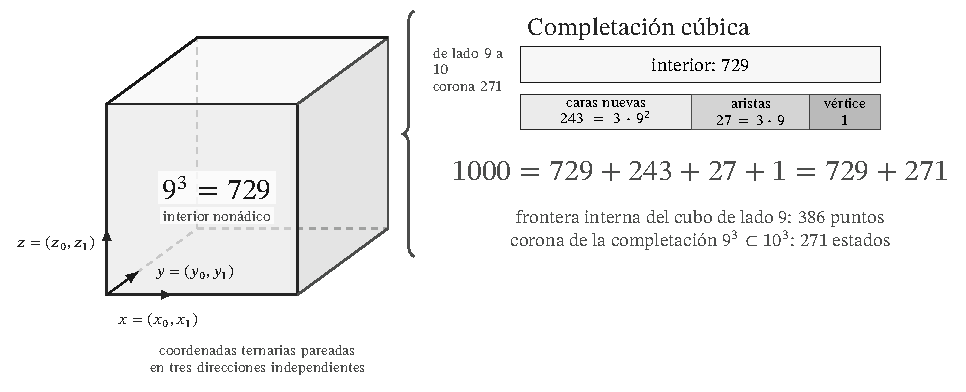
\includegraphics[width=\linewidth]{figures/cubo_emrh.pdf}
\caption{Representación cúbica de la ampliación de nueve a diez clases por coordenada. Los estratos \(S_1,S_2,S_3\) sitúan las incidencias añadidas en caras, aristas y ápice; sus cardinales forman la corona de \(271\) elementos. La frontera de \(386\) elementos pertenece al cubo inicial. La perspectiva geométrica complementa la partición de la figura~\ref{fig:revision-emrh}; las separaciones gráficas tienen función esquemática.}
\label{fig:completacion-cubo-recuperado}
\end{figure}
